\documentclass[conference]{IEEEtran}

% =========================================================
% PAQUETES
% =========================================================

\usepackage[utf8]{inputenc}
\usepackage[T1]{fontenc}
\usepackage[spanish,es-nodecimaldot]{babel}

\usepackage{amsmath}
\usepackage{amssymb}

\usepackage{graphicx}
\usepackage{float}

\usepackage{booktabs}
\usepackage{array}

\usepackage{siunitx}

\usepackage{cite}

\usepackage{url}

% Para código
\usepackage{listings}



\renewcommand{\IEEEkeywordsname}{Palabras clave}


\begin{document}



\title{
CRITERIO DE NYQUIST-SHANNON Y ALIASING EN LA CONVERSIÓN DE SEÑALES ANALÓGICAS A DIGITALES
}


\author{
\IEEEauthorblockN{
Jefferson Velasquez, 
Sneider Sanabria,
Daniela Calderón 
}

\IEEEauthorblockA{
Ingeniería Electrónica\\
Universidad de los Llanos\\
Villavicencio, Colombia\\
jevelasquez.quevedo@correo.com,
sy.salfonzo@unillanos.edu.co,
dscalderon.moreno@unillanos.edu.co
}
}

\maketitle



\begin{abstract}

En este trabajo se presenta el análisis experimental de los procesos de muestreo
y reconstrucción de señales analógicas, dónde se evaluó el cumplimiento 
del teorema de muestreo de Nyquist-Shannon y el fenómeno de aliasing. Se 
implementó un circuito oscilador basado en el temporizador NE555 y el interruptor 
bilateral CD4066, mediante el cual se obtuvieron muestras de una señal senoidal de 
5 kHz a diferentes frecuencias de muestreo. Posteriormente, se incorporó un circuito,
conformado por un filtro pasabajas RC y un seguidor de voltaje, 
con el objetivo de reconstruir la señal muestreada. Los resultados medidos mediante el
osciloscopio permitió comparar la señal original contra la señal reconstruida, en cada 
condición de muestreo, se evidenció que la reconstrucción con una frecuencia de muestreo de $F_s\approx\SI{300}{\kilo\hertz}$
es la que más se aproxima a la señal original, cumpliendo con el criterio de Nyquist-Shannon.

\end{abstract}


\begin{IEEEkeywords}

Aliasing, muestreo, retención, reconstrucción de señales, teorema de Nyquist-Shannon.

\end{IEEEkeywords}


\section{Introducción}

En los sistemas electrónicos y de control es frecuente trabajar con señales analógicas que deben ser procesadas mediante dispositivos digitales. Un sistema en tiempo discreto se define como un sistema que recibe una secuencia de valores de entrada $x[n]$ y la transforma en una secuencia de valores de salida $y[n]$ \cite{oppenheim}. Estos sistemas son dinámicos y sus variables pueden cambiar únicamente en determinados instantes, conocidos como muestreo \cite{cuero}. El muestreo se define como el proceso mediante el cual se representa una señal continua a través de un conjunto de muestras tomadas en determinados instantes de tiempo. La selección adecuada de la frecuencia de muestreo es necesaria para conservar la información contenida en la señal original \cite{ogata}.

El teorema de muestreo de Nyquist--Shannon establece que una señal limitada en banda puede ser reconstruida a partir de sus muestras cuando la frecuencia mínima de muestreo es, como mínimo, el doble de su máxima componente frecuencial. Cuando esta condición no se cumple, se produce un fenómeno denominado aliasing \cite{semeria}, en el cual diferentes componentes de frecuencia de la señal original pueden generar representaciones indistinguibles en la señal muestreada, provocando una pérdida de información durante el proceso de digitalización \cite{osorio}.

Además del muestreo, en la conversión de señales que tiene lugar en el sistema de control digital, se requiere una etapa de retención, cuya función es mantener el valor del pulso obtenido durante el proceso de muestreo durante un tiempo específico \cite{ogata}. El muestreador permite obtener la señal en instantes $(0, T, 2T, \ldots)$, donde $T$ corresponde al periodo de muestreo, mientras que el retenedor permite mantener el valor de cada muestra hasta el siguiente instante de muestreo. El retenedor más fundamental es el retenedor de orden cero, el cual mantiene constante el valor de la muestra entre dos instantes de muestreo consecutivos; la precisión de la reconstrucción mediante este tipo de retenedor depende de la magnitud del periodo de muestreo \cite{cuero}.

Por lo anterior, la presente práctica de laboratorio tiene como objetivo analizar experimentalmente los procesos involucrados en la conversión de señales analógicas a digitales mediante el muestreo, retención y la reconstrucción de una señal. Para ello, se implementará un circuito de muestreo utilizando un temporizador NE555 y un interruptor bilateral CD4066, mediante los cuales se obtendrán muestras de una señal senoidal a diferentes frecuencias de muestreo. Posteriormente, se incorporará un circuito retenedor conformado por un filtro RC y un seguidor de voltaje, con el propósito de observar el comportamiento de la señal reconstruida. Finalmente, se analizaran las señales obtenidas mediante el osciloscopio, relacionando los resultados experimentales con los fundamentos del teorema de Nyquist - Shannon y el fenómeno del aliasing.


% =========================================================
% II. FUNDAMENTO TEÓRICO
% =========================================================

\section{Fundamento teórico}


Los sistemas de control en tiempo discreto difieren de los continuos en que sus variables varían únicamente en instantes específicos \cite{ogata}. 
El muestreo periódico de una señal analógica $x_a(t)$ permite obtener una secuencia en tiempo discreto $x(n)$, definida por la relación:
\begin{equation}
    x(n) = x_a(nT)
\end{equation}
Donde $T$ es el periodo de muestreo. Para comprender este proceso es importante analizar el comportamiento de la señal tanto en el dominio del tiempo como en el dominio de la frecuencia \cite{fadali}.

\subsection{Teorema del Muestreo y Criterio de Nyquist-Shannon}

El Criterio de Nyquist-Shannon establece que, para recuperar exactamente una señal analógica de ancho de banda limitado a partir de sus muestras,
la frecuencia de muestreo ($f_s$) debe ser estrictamente mayor que el doble de la frecuencia máxima contenida en la señal ($f_{max}$) \cite{garcia}. Matemáticamente, esto se expresa como:
\begin{equation}
    f_s > 2f_{max}
\end{equation}

Si esta condición no se cumple, las réplicas del espectro de la señal en el dominio de la frecuencia se solapan. Este fenómeno,
conocido como \textit{aliasing} (o solapamiento), produce componentes de baja frecuencia espurias en la señal reconstruida que no existían en la señal analógica original,
lo que imposibilita la reconstrucción exacta por parte del circuito retenedor \cite{alvarado}.

\subsection{Análisis en el Dominio de la Frecuencia y la Transformada Rápida de Fourier (FFT)}

En la instrumentación electrónica moderna, este proceso se ejecuta computacionalmente mediante el algoritmo de la Transformada Rápida de Fourier (FFT). 
Esta misma reduce drásticamente la complejidad computacional del análisis espectral, permitiendo a osciloscopios digitales con capacidades avanzadas\cite{astrom}.

\subsection{Espectro de Frecuencia y Armónicos en la Retención}

Cuando una señal senoidal analógica es muestreada por un interruptor bilateral (como el CD4066) controlado por un tren de pulsos (generado, por ejemplo,
mediante un multivibrador astable NE555), la operación equivale matemáticamente a la multiplicación de la señal original por un tren de impulsos periódico \cite{ogata}.

En el dominio de la frecuencia, esta multiplicación se traduce en la convolución del espectro de la señal original con el espectro del tren de pulsos.
Como resultado, el espectro de la señal muestreada contiene la frecuencia fundamental original y un número infinito de réplicas exactas (armónicos) centradas alrededor de los múltiplos de la frecuencia de muestreo ($f_s, 2f_s, 3f_s, \dots$) \cite{alvarado}.

\section{Metodología}

 Inicialmente se diseñó un circuito multivibrador astable, dónde se usó 
el integrado NE555 en su configuración astable para generar una señal de onda cuadrada 
periódica, esta señal se utilizó para
determinar el tiempo de muestreo en un rango aproximado de 1k Hz hasta 50k Hz.
La señal proveniente del NE555 se conectó a la entrada de control (pin 13) de un interruptor bilateral 
del circuito integrado CD4066, a la entrada del interruptor (pin 1) se conectó 
una señal sinusoidal con amplitud de 5 Vpp, offset de 5 V y frecuencia de 5 kHz proveniente de un generador de señales. 
A la salida del muestreador (pin 2) se conectó una resistencia de carga RL a tierra,
mediante el osciloscopio se registró el comportamiento de la señal en RL
al variar la frecuencia de muestreo del NE555.
La señal del chip CD4066 en el pin 2 se acondicionó con un filtro pasabajas pasivo RC.

Finalmente se agregó a la salida del filtro un amplificador operacional en su configuración seguidor de voltaje,
al comprobar el funcionamiento del circuito en el software de simulación de Multisim, se implementó 
el circuito de manera experimental. Por medio del osciloscopio se observó el comportamiento de la señal a las diferencias frecuencias de muestreo
dónde se comparó la señal original con la señal reconstruida.  


\subsection{Simulación en el software Multisim}

Se realizó la simulación del circuito correspondiente a la generación de la señal de muestreo.
La Fig.~\ref{fig:NE555} presenta el integrado NE555 en su configuración de oscilador astable, mediante el potenciometro de 100 k$\Omega$
se configura la frecuencia de muestreo.

\begin{figure}[H]
    \centering
    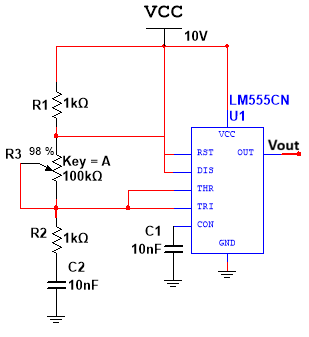
\includegraphics[width=0.5\columnwidth]
    {imagenes/NE555.png}
    \caption{Simulación del circuito que genera la señal de muestreo con el NE555.}
    \label{fig:NE555}
\end{figure}


La Fig.~\ref{fig:CD4066} muestra la simulación completa en el software Multisim, donde se  observa la conexión 
de la señal de muestreo al pin 13 del CD4066, posteriormente la señal de salida en el pin 2 se conecta a un filtro RC 
y al seguidor de voltaje, finalmente se observa la señal de salida en la resistencia de carga RL.

\begin{figure}[H]
    \centering
    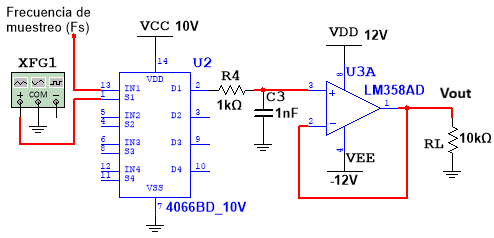
\includegraphics[width=0.7\columnwidth]
    {imagenes/CD4066.png}
    \caption{Simulación del circuito integrado CD4066, filtro RC, seguidor de voltaje y generador de señales.}
    \label{fig:CD4066}
\end{figure}



\subsection{Implementación experimental}

Se implementó el circuito de manera experimental, dónde se verificó el funcionamiento de cada etapa,
desde la generación de la señal de muestreo, hasta la salida del amplificador operacional en su configuración seguidor de voltaje. 


\begin{figure}[H]
    \centering
    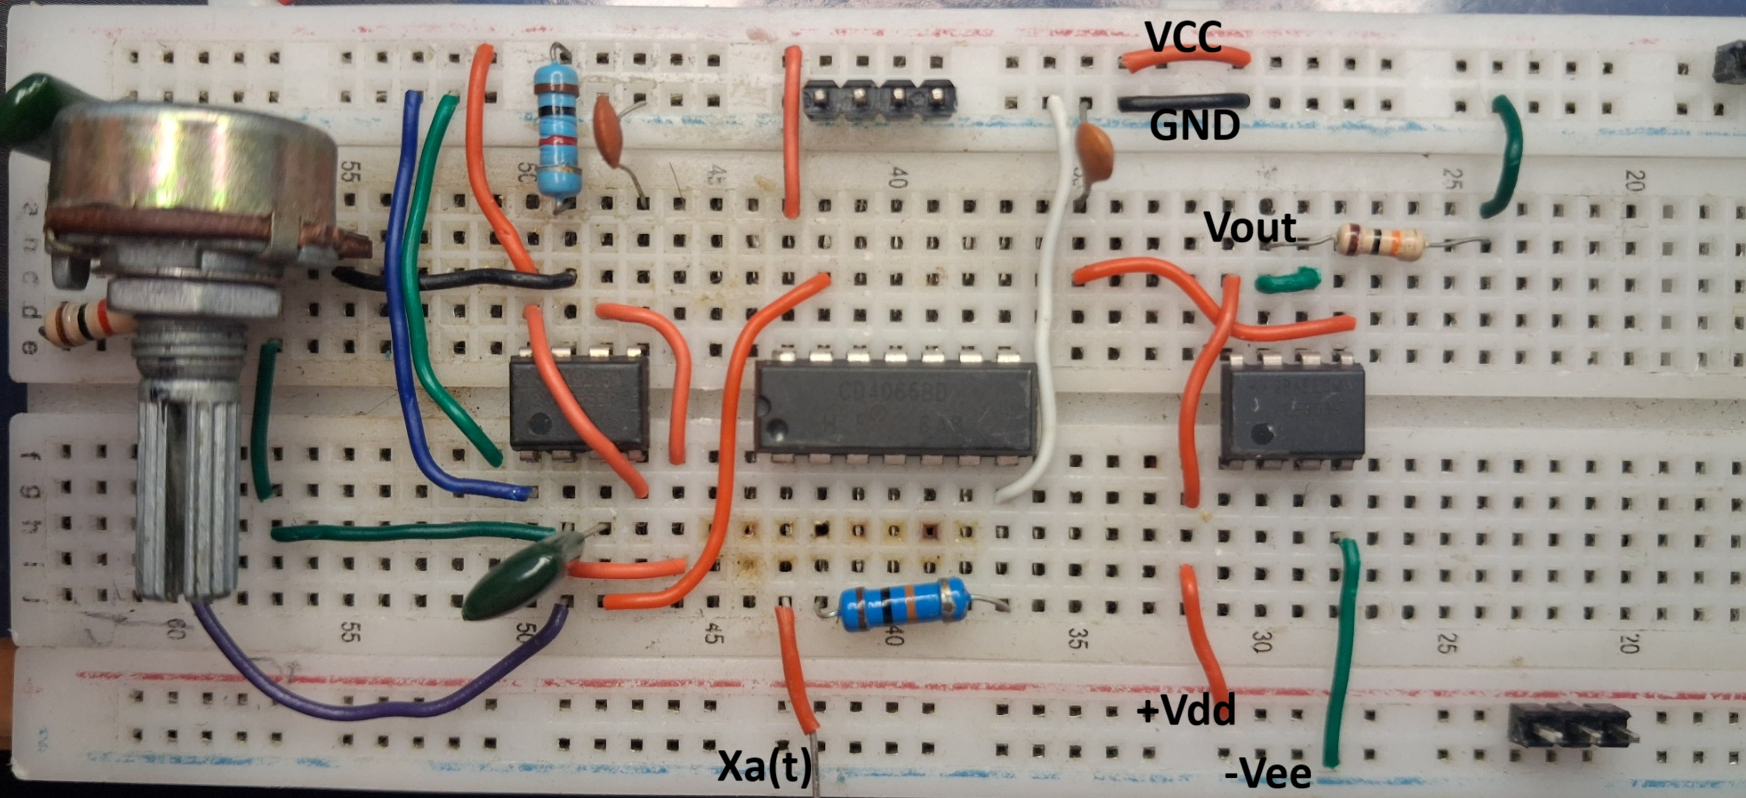
\includegraphics[width=0.7\columnwidth]
    {imagenes/montaje.png}
    \caption{Montaje físico en protoboard de cada etapa diseñada en simulación.}
    \label{fig:montaje}
\end{figure}

En la figura \ref{fig:montaje} se observa Xa(t) la señal análogica de entrada correspondiente a una señal sinusoidal.

Dónde:

\begin{itemize} 
\item VCC: Voltaje de alimentación para el NE555 y CD4066.
\item GND: Tierra común de todo el circuito. 
\item +VDD: Voltaje de alimentación para el amplificador operacional. 
\item -VEE: Voltaje de alimentación negativo del amplificador operacional.
\end{itemize}


% =========================================================
% IV. RESULTADOS
% =========================================================
\section{Resultados}

\subsection{Resultados experimentales}

Al variar la frecuencia de muestreo $F_s$ generada por el circuito NE555, se observó
que la forma de la señal en $R_L$ dependía directamente de la relación entre $F_s$
y la frecuencia de la señal analógica de entrada ($f_{x_a} = 5$ kHz). Para valores
bajos de $F_s$, la señal muestreada y reconstruida presentó distorsión,
alejándose considerablemente de la forma senoidal original, evidenciando el fenómeno
de aliasing descrito por el teorema de Nyquist--Shannon. A medida que $F_s$ aumentó
y superó el doble de la frecuencia de la señal de entrada (criterio de Nyquist,
$F_s \geq 2f_{x_a} = 10$ kHz), la señal reconstruida comenzó a aproximarse
progresivamente a la señal original para las frecuencias de muestreo más altas evaluadas
(\SI{170}{\kilo\hertz} y \SI{300}{\kilo\hertz}), como se observa en la figura \ref{fig:comparacion}. 



\begin{figure}[H]
    \centering
    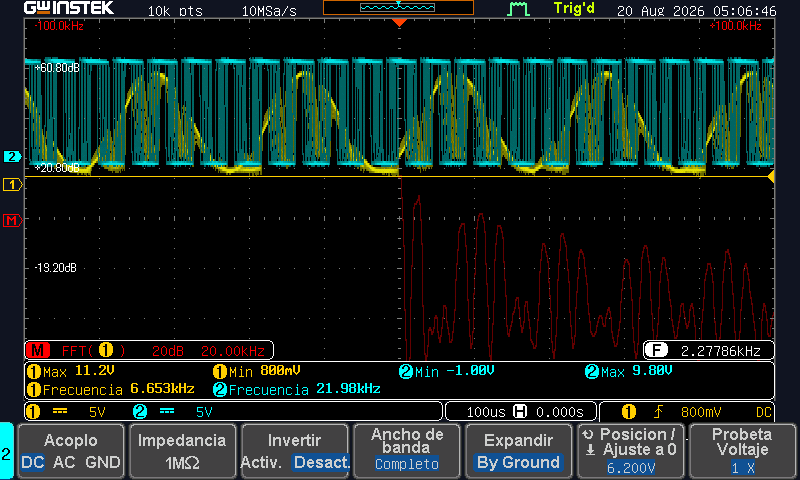
\includegraphics[width=0.48\columnwidth]{imagenes/four.PNG}
    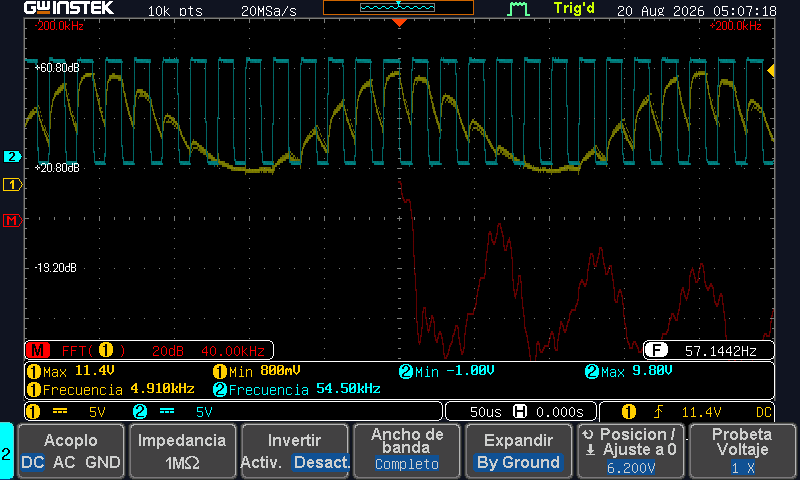
\includegraphics[width=0.48\columnwidth]{imagenes/tre.PNG}
    \\[0.3em]
    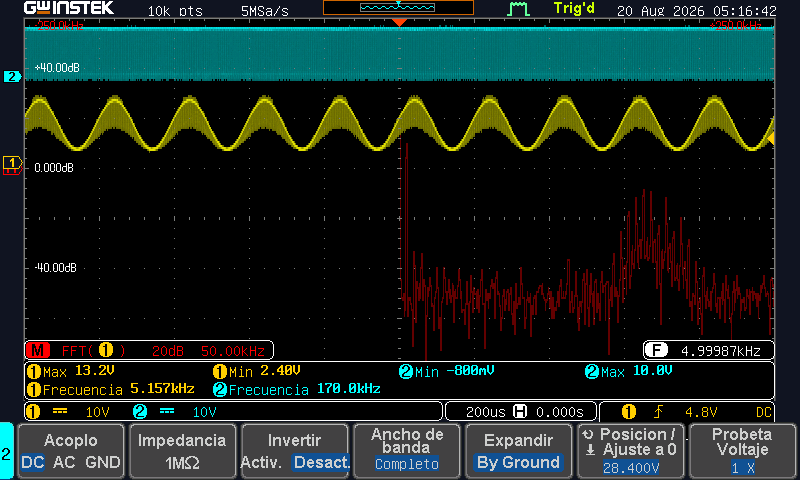
\includegraphics[width=0.48\columnwidth]{imagenes/two.PNG}
    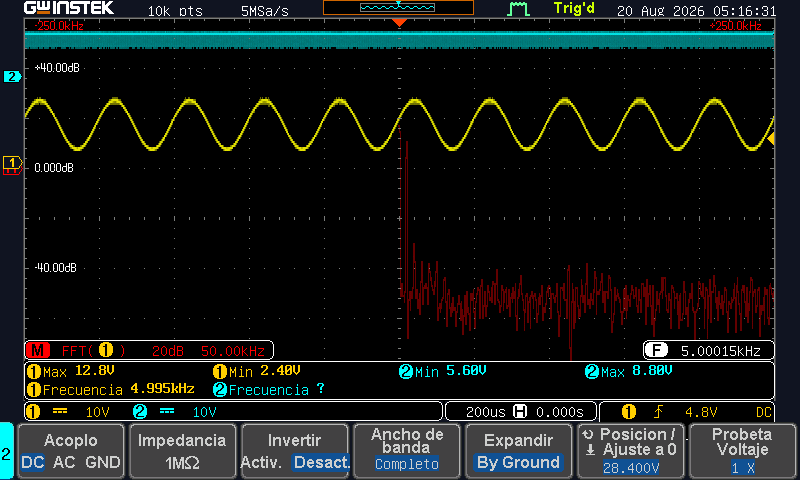
\includegraphics[width=0.48\columnwidth]{imagenes/one.PNG}

    \caption{Evolución de la señal reconstruida con
    $F_s=\SI{21.9}{\kilo\hertz}$,
    $F_s=\SI{54.5}{\kilo\hertz}$,
    $F_s=\SI{170}{\kilo\hertz}$ y
    $F_s\approx\SI{300}{\kilo\hertz}$ respectivamente.}

    \label{fig:comparacion}
\end{figure}

Posteriormente se obtuvo el espectro de la señal secontruida, mediante la transformada rápida de fourier (FFT)
por medio de la función math en el osciloscopio.

El espectro de la señal en la figura \ref{fig:fft1}, se observa ármonicos que son múltiplos enteros de la frecuencia alrededor 
de la frecuencia fundamental, debido a la distorsión generada por el aliasing y una frecuencia de muestreo insuficiente. 

\begin{figure}[H]
    \centering
    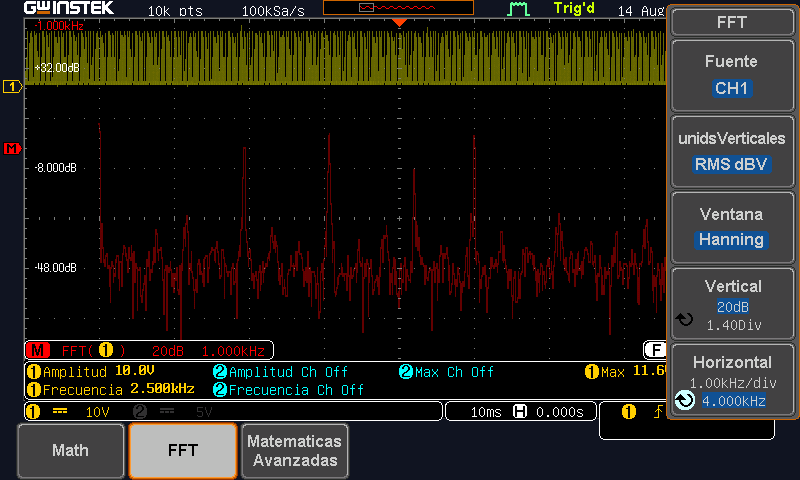
\includegraphics[width=0.7\columnwidth]
    {imagenes/FFT1.png}
    \caption{Armónicos presentes en la señal reconstruida con una frecuencia de muestreo de \SI{2.5}{\kilo\hertz}.}
    \label{fig:fft1}
\end{figure}

Al incrementar la frecuencia de muestreo, los ármonicos presentes en la figura \ref{fig:fft1}
se van a alejando de la frecuencia fundamental de la señal reconstruida, permitiendo observar en la figura \ref{fig:fft} 
un único pico referente a la frecuencia real de la señal.

\begin{figure}[H]
    \centering
    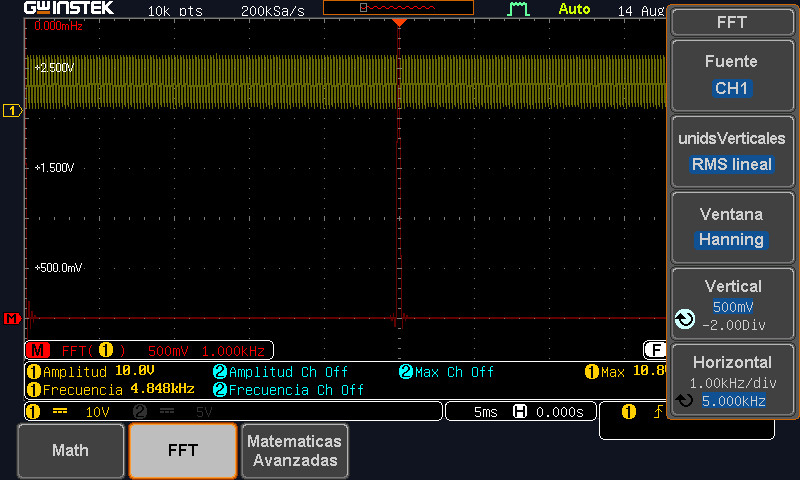
\includegraphics[width=0.7\columnwidth]
    {imagenes/FFT.png}
    \caption{Espectro de la señal obtenida mediante la función math del osciloscopio.}
    \label{fig:fft}
\end{figure}


% =========================================================
% VII. CONCLUSIONES
% =========================================================

\section{Conclusiones}

\begin{itemize}

    \item Se logró implementar el sistema propuesto
    de acuerdo con los objetivos establecidos.

    \item Los resultados experimentales permitieron
    verificar el comportamiento esperado del sistema.

    \item Se identificaron las principales fuentes
    de error y sus efectos sobre las mediciones.

\end{itemize}


% =========================================================
% REFERENCIAS
% =========================================================

\begin{thebibliography}{00}
\bibitem{oppenheim}
A. V. Oppenheim, R. W. Schafer y J. R. Buck,
\textit{Tratamiento de señales en tiempo discreto}, 2011.

\bibitem{cuero}
J. D. Cuero,
``Práctica No. 01: Muestreo, retención y reconstrucción de señales muestreadas,''
guía de laboratorio, Universidad de los Llanos, Facultad de Ingeniería Electrónica, 2017.

\bibitem{ogata}
K. Ogata,
\textit{Sistemas de Control en Tiempo Discreto}, 2.ª ed.

\bibitem{semeria}
M. Semeria,
``Los tres teoremas: Fourier-Nyquist-Shannon,''
Serie Documentos de Trabajo, no. 582, 2015.

\bibitem{osorio}
J. A. C. Osorio, H. B. C. Garzón y J. A. C. Osorio,
``Fundamentos y aplicación del muestreo en señales ubicadas en las bandas altas del espectro,''
\textit{Scientia Et Technica}, vol. 14, no. 39, pp. 37--42, 2008.

\end{thebibliography}


\end{document}